\documentclass{beamer}
\usetheme{Darmstadt}
\usepackage{comment}
\usepackage[utf8]{inputenc}    % Para escribir acentos y caracteres especiales
\usepackage{graphicx}          % Para insertar imágenes
\usepackage{booktabs}          % Para tablas más bonitas
\usepackage{amsmath}           % Para escribir ecuaciones
\usepackage{tikz}              % Para gráficos vectoriales
\usetikzlibrary{calc}          % Para coordenadas calculadas con TikZ
\usepackage{pgfplots}          % Para gráficos matemáticos
\pgfplotsset{compat=1.18}      % Evita errores por compatibilidad

\title{Ayudantía 1 \\ Bonos \\ \large\textit{Instrumentos Derivados}}
\author{
  \texorpdfstring{
    \textbf{Profesor:} Francisco Rantul \\[0.3em]
    \textbf{Ayudante:} Mateo Canales
  }{Profesor: Francisco Rantul, Ayudante: Mateo Canales}
}
\subject{Instrumentos Derivados}
\institute{Universidad Diego Portales}
\date{31 De Marzo, 2025}

\begin{document}

% Portada
\begin{frame}
    \titlepage
    \vfill
    \centering
    
\includegraphics[width=2.3118cm]{../imagenes/logo.png}
  \end{frame}
\begin{frame}
  \frametitle{Contenido}
  \tableofcontents
\end{frame}

\section{Materia}
  \begin{frame}

  \sectionpage   
  \end{frame}  

%ejemplo ecuaciones
\begin{frame}
    \frametitle{Cálculo de Bonos}
    Una fórmula conocida:
    \[
        E = mc^2
        \]
        
        Otra ecuación inline: \( a^2 + b^2 = c^2 \)
\end{frame}
% Gráfico Sin(x)
\begin{frame}
  \frametitle{Gráfico PGFPlots}
  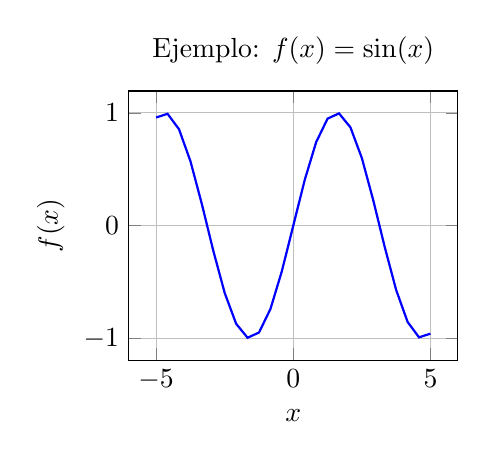
\begin{tikzpicture}
    \begin{axis}[
        width=6.5cm, scale=0.85, clip=true,
        xlabel={$x$},
        ylabel={$f(x)$},
        title={Ejemplo: $f(x)=\sin(x)$},
        grid=major,
        ]
        \addplot[blue, thick] {sin(deg(x))};
    \end{axis}
  \end{tikzpicture}
  \end{frame}
\section{Ejercicios}
\begin{frame}
    \centering
    \Huge \insertsection
\end{frame}
\begin{frame}
  \frametitle{Ejercicio 1 A$)$}
  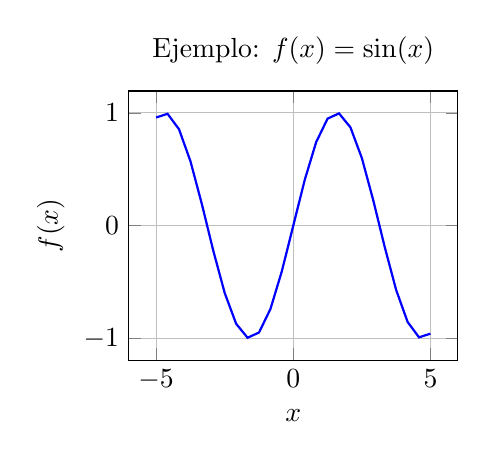
\begin{tikzpicture}
    \begin{axis}[
        width=6.5cm, scale=0.85, clip=true,
        xlabel={$x$},
        ylabel={$f(x)$},
        title={Ejemplo: $f(x)=\sin(x)$},
        grid=major,
        ]
        \addplot[blue, thick] {sin(deg(x))};
    \end{axis}
  \end{tikzpicture}
  \end{frame}
\end{document}